\documentclass{ieeeaccess}
\usepackage{cite}
\usepackage{amsmath,amssymb,amsfonts}
\usepackage{algorithmic}
\usepackage{graphicx}
\usepackage{textcomp}

\def\BibTeX{{\rm B\kern-.05em{\sc i\kern-.025em b}\kern-.08em
    T\kern-.1667em\lower.7ex\hbox{E}\kern-.125emX}}
\begin{document}
\history{Date of publication xxxx 00, 0000, date of current version xxxx 00, 0000.}
\doi{10.1109/ACCESS.2020.DOI}

\title{Preparation of Papers for IEEE ACCESS}
\author{\uppercase{Michael Zhang}\authorrefmark{1}, \IEEEmembership{Student Member, IEEE},
\uppercase{Chandra Krintz}\authorrefmark{1}, \IEEEmembership{Member, IEEE}, \uppercase{Rich Wolski}.\authorrefmark{1},
\IEEEmembership{Member, IEEE}}
\address[1]{Racelab, University of California, Santa Barbara, CA  93106-5110 U.S.A}

\tfootnote{This work has been supported in part by NSF (CNS-1703560, CCF-1539586,
ACI-1541215), ONR NEEC (N00174-16-C-0020),
and the AWS Cloud Credits for Research program.}

\markboth
{Author \headeretal: STOIC CPSS Paper}
{Author \headeretal: STOIC CPSS Paper}

\corresp{Corresponding author: Michael Zhang (e-mail: lebo@cs.ucsb.edu).}

\begin{abstract}
\label{sec:abstract}
abstract
\end{abstract}

\begin{keywords}
% Enter key words or phrases in alphabetical 
% order, separated by commas. For a list of suggested keywords, send a blank 
% e-mail to keywords@ieee.org or visit \underline
% {http://www.ieee.org/organizations/pubs/ani\_prod/keywrd98.txt}
Edge computing, Image Processing, Internet of Things, Serverless computing
\end{keywords}

\titlepgskip=-15pt

\maketitle

\section{Introduction}
\label{sec:introduction}
Introduction

\section{STOIC}
\label{sec:STOIC}
STOIC


\section{Evaluation}
\label{sec:eval}
Result

\section{Related Work}
\label{sec:relate_work}
Related Work


\section{Conclusion}
\label{sec:conclusion}
Conclusion

\section*{Acknowledgment}
This work has been supported in part by NSF (CNS-1703560, CCF-1539586,
ACI-1541215), ONR NEEC (N00174-16-C-0020),
and the AWS Cloud Credits for Research program.

\begin{thebibliography}{00}

\bibitem{b1} G. O. Young, ``Synthetic structure of industrial plastics,'' in \emph{Plastics,} 2\textsuperscript{nd} ed., vol. 3, J. Peters, Ed. New York, NY, USA: McGraw-Hill, 1964, pp. 15--64.
\end{thebibliography}


\begin{IEEEbiography}[{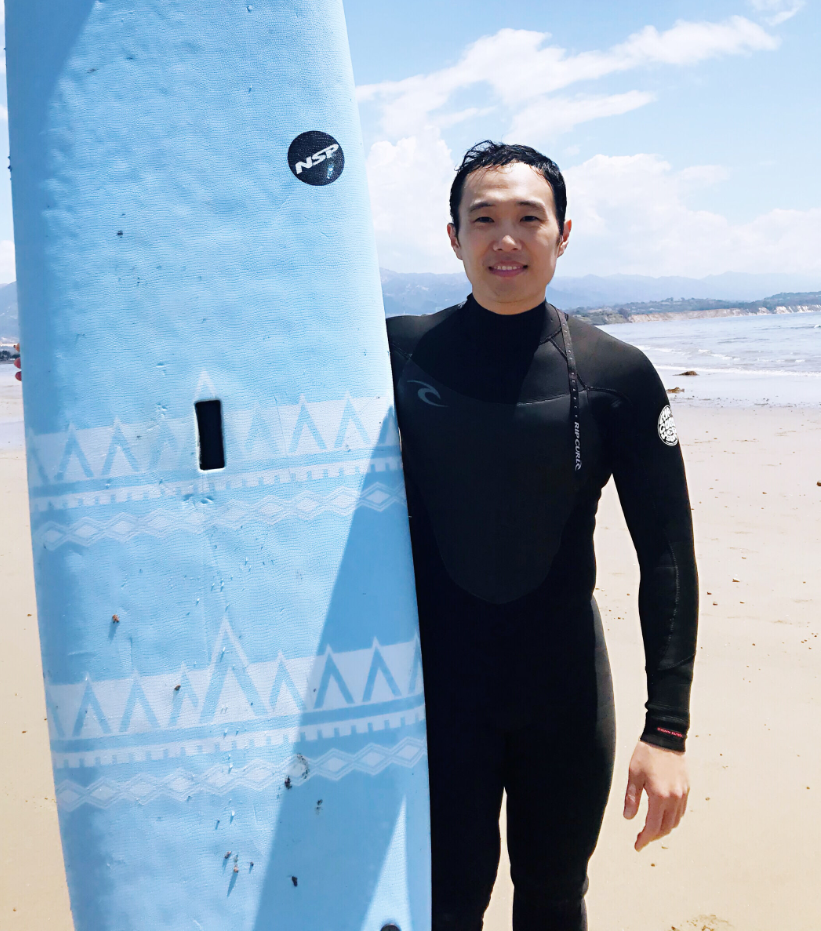
\includegraphics[width=1.1in,height=1.5in,clip,keepaspectratio]{figures/a1.png}}]{Michael Zhang} (M'76--SM'81--F'87) and all authors may include 
biographies. Biographies are often not included in conference-related
papers. This author became a Member (M) of IEEE in 1976, a Senior
Member (SM) in 1981, and a Fellow (F) in 1987. The first paragraph may
contain a place and/or date of birth (list place, then date). Next,
the author's educational background is listed. The degrees should be
listed with type of degree in what field, which institution, city,
state, and country, and year the degree was earned. The author's major
field of study should be lower-cased. 


\end{IEEEbiography}

\begin{IEEEbiography}[{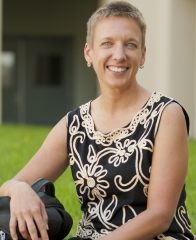
\includegraphics[width=1in,height=1.25in,clip,keepaspectratio]{figures/a2.png}}]{Chandra Krintz} was born in Greenwich Village, New York, NY, USA in 
1977. He received the B.S. and M.S. degrees in aerospace engineering from 
the University of Virginia, Charlottesville, in 2001 and the Ph.D. degree in 
mechanical engineering from Drexel University, Philadelphia, PA, in 2008.

\end{IEEEbiography}

\begin{IEEEbiography}[{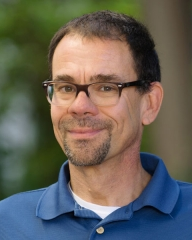
\includegraphics[width=1in,height=1.25in,clip,keepaspectratio]{figures/a3.png}}]{Rich Wolski} (M'87) received the B.S. degree in mechanical 
engineering from National Chung Cheng University, Chiayi, Taiwan, in 2004 
and the M.S. degree in mechanical engineering from National Tsing Hua 
University, Hsinchu, Taiwan, in 2006. He is currently pursuing the Ph.D. 
degree in mechanical engineering at Texas A{\&}M University, College 
Station, TX, USA.

\end{IEEEbiography}


\EOD

\end{document}
